\part*{Ejercicio 1}
Se nos pidió diseñar e implementar una maquina de estados capaz de controlar la activación de dos bombas B1 y B2 (simulando su encendido con un LED) que deben mantener el nivel de agua de un depósito que dispone de dos sensores S e I, colados en la parte superior e inferior del depósito, respectivamente. La operatoria de la máquina sigue las siguientes reglas:

\begin{itemize}
\item Si el agua ha superado un sensor, su valor de salida será: 1.
\item Si el deposito estuviera lleno (I=S=1) no se activaría ninguna bomba.
\item Si el deposito estuviera vacío (I=S=0) se activarían ambas bombas.
\item Si el deposito estuviera lleno por la mitad (I=1, S=0) se activaría la ultima bomba en no activarse. 
\end{itemize}

Se nos solicitó tener en cuenta las siguientes consideraciones para la implementación de la maquina de estados:

\begin{itemize}
\item Implementar la solución utilizando tanto una maquina de Mealy como de Moore.
\item Muestre claramente el diagrama de estados y transiciones.
\item Respaldar el diseño con una simulación en Verilog.
\end{itemize} 

Se debe mencionar que en ambas implementaciones(Moore y Mealy) se utilizó un Flip-Flop JK en modo toggle para implementar el alternado de las bombas. La lógica secuencial del Flip-Flop en cuestión es función solo de los estados de la máquina, y no del clock directamente (como si lo son los Flip-Flops que almacenan el estado actual de la maquina), por lo tanto se consideró apropiada tal implementación aún no cumpliendo con la definición estricta de máquina de estados de Moore y Mealy, que dice que la salida es una lógica combinacional de los estados (y las entradas en el caso de Mealy). Puede considerarse este Flip-Flop JK en modo toggle que controla el alternado de las salidas como una maquina de estados englobada por otra. 

\section*{Implementación Maquina de Moore}
\subsection*{Diagrama de Estados y Transiciones}

Se comenzó por la implementación de la máquina de estados de Moore, para ello, se comenzó por realizar un diagrama de estados y transiciones que describa la maquina de estados. Para lo cual se listará primero a las entradas, estados y salidas posibles, y se hará una breve descripción para una mejor comprensión del diagrama.

\subsubsection*{Entradas:}

\begin{description}
\item[Vacío:] Configuración de entrada S=0, I=0, que indica que el depósito se encuentra vacío.
\item[Medio:] Configuración de entrada S=0, I=1, que indica que el depósito esta lleno por la mitad.
\item[Lleno:] Configuración de entrada S=1, I=1, que indica que el depósito se encuentra lleno.
\end{description}

\subsubsection*{Estados:}

\begin{description}
\item[Ninguna:] Estado que indica que ninguna bomba esta encendida.
\item[Una Sola:] Estado que indica que solo una bomba se encuentra encendida.
\item[Ambas:] Estado que indica que ambas bombas se encuentran encendidas.
\end{description}

\subsubsection*{Salidas:}

\begin{description}
\item[$b_1=0$ y $b_2=0$:] Esta configuración de salida no enciende ninguna bomba.
\item[$b_1=1$,$b_2=0$ o $b_1=0$,$b_2=1$:] Solo se enciende una de las bombas que controla el circuito.
\item[$b_1=1$ y $b_2=1$:] Esta configuración de salida enciende las dos bombas.
\end{description}

A continuación se presenta el diagrama de estados y transiciones, a partir del cual se diseñó la maquina de estados:

\begin{figure}[H]
\centering
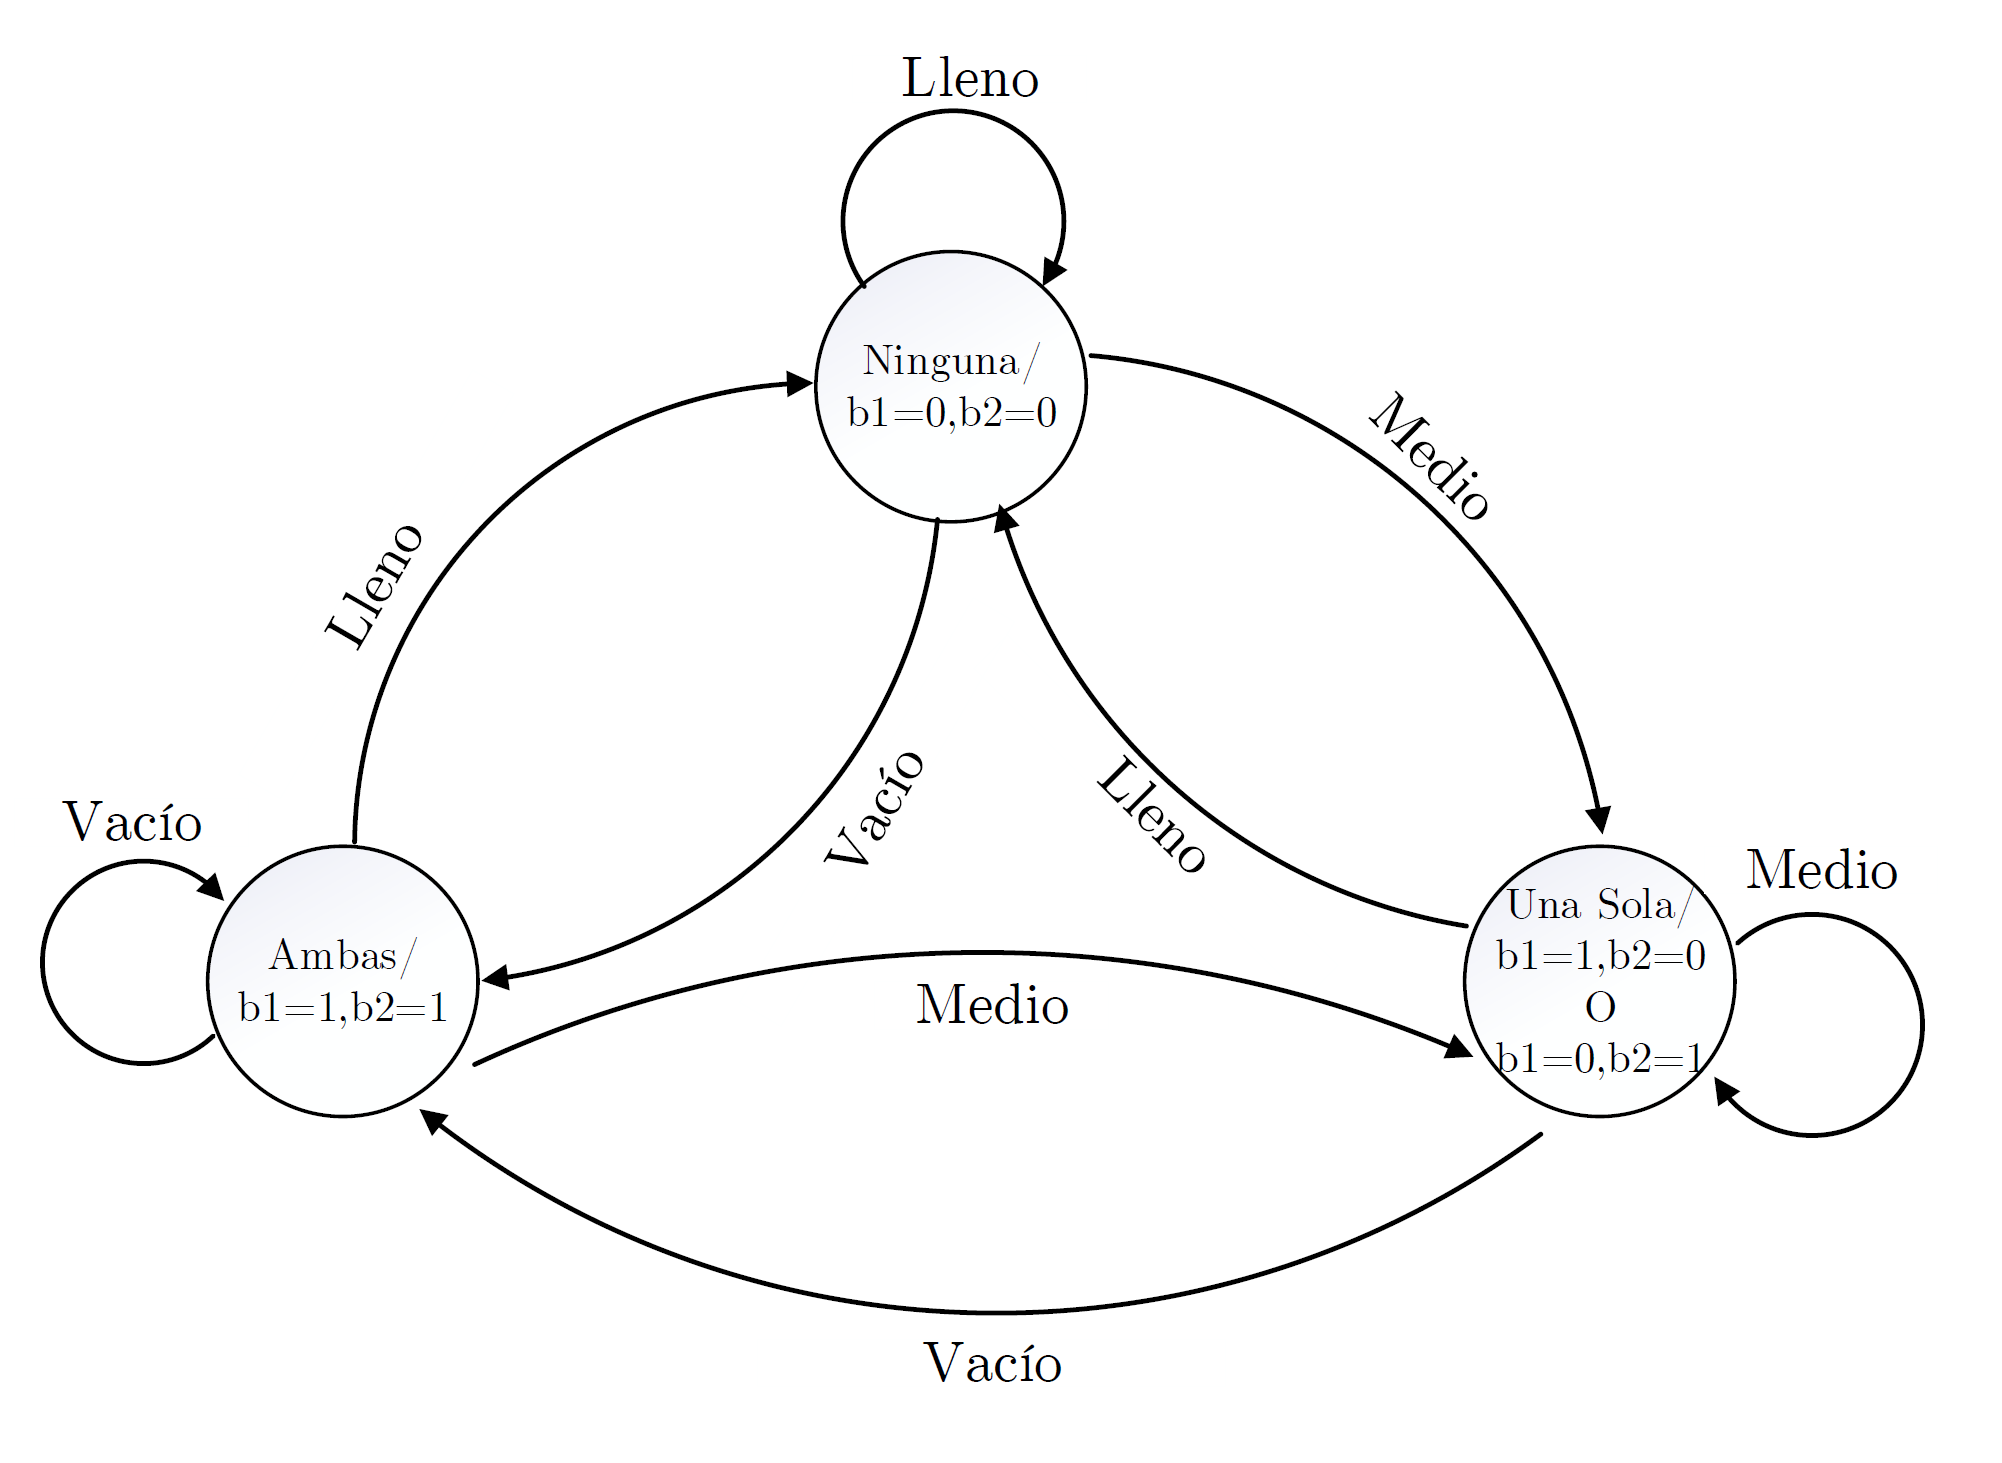
\includegraphics[scale=0.3]{images/diagrama_estados_moore.png}
\caption{Diagrama de estados y transiciones} \label{1_figa}
\end{figure}

Al contar con 3 estados diferentes, mi maquina de estados necesitará como mínimo dos Flip-Flop's para almacenar el estado actual. Los tres estados posibles se codifican a traves de dos variables $y_1$ e $y_0$, de esta forma, tendremos las siguientes configuraciones:

\bigskip

\begin{table}[ht]
	\centering
	\begin{tabular}{c|c}
	Estado & $y_1y_0$ \\ 
	\hline 
	Ninguna & 00 \\ 
	Una Sola & 01 \\ 
	Ambas & 11 \\ 
	\end{tabular} 
\end{table}


Habiendo definido los estados del diseño, se procedió a completar la correspondiente tabla de asignación de estados:
\bigskip
\begin{table}[ht]
	\centering
	\begin{tabular}{c|c|c|c|c}
	Estado Actual & \multicolumn{3}{c|}{Próximo Estado$(Y_1Y_0)$} & Salida\\
	\cline{2-4}
	$(y_1y_0)$ & $SI=00$ & $SI=01$ & $SI=11$ & $(b_1b_2)$\\
	\hline
	00 & 11 & 01 & 00 & 00 \\
	01 & 11 & 01 & 00 & 01 o 10 (Alternado) \\
	11 & 11 & 01 & 00 & 11 \\
	\end{tabular}
	\caption{Tabla de asignación de estados}
	\label{1_t1}
\end{table}

A partir del Cuadro \ref{1_t1} se confeccionó el Cuadro \ref{1_t2}, que implementa la tabla de verdad que determina el próximo estado ($Y_1Y_0$) en función del estado anterior ($y_1y_0$) y las entradas ($SI$). 



\begin{table}[H]
	\centering
	\begin{tabular}{c|c|c}
	$y_1y_0SI$ & $Y_1$ & $Y_0$  \\ 
	\hline 
	0000 & 1 & 1  \\ 
	\hline 
	0001 & 0 & 1  \\ 
	\hline 
	0010 & x & x  \\ 
	\hline 
	0011 & 0 & 0  \\ 
	\hline 
	0100 & 1 & 1  \\ 
	\hline 
	0101 & 0 & 1  \\ 
	\hline 
	0110 & x & x  \\ 
	\hline 
	0111 & 0 & 0  \\ 
	\hline 
	1000 & x & x  \\ 
	\hline 
	1001 & x & x  \\ 
	\hline 
	1010 & x & x  \\ 
	\hline 
	1011 & x & x  \\ 
	\hline 
	1100 & 1 & 1  \\ 
	\hline 
	1101 & 0 & 1  \\ 
	\hline 
	1110 & x & x  \\ 
	\hline 
	1111 & 0 & 0  \\ 
	\end{tabular} 
	\caption{Tabla de verdad cambio de estado}
	\label{1_t2}
\end{table}

Se determinó que es estado $SI=10$ no es una combinación posible, ya que indicaría que el agua ha superado el sensor superior pero no el inferior, lo cual es incompatible con el modelo del deposito, e indicaría un error en los sensores. Como el manejo de errores en el sensores excede los requisitos de la consigna es que se determinó que no son combinaciones posibles y las salidas correspondientes a estas configuraciones se determinaron como 'don't care'

La simplificación mediante Mapas de Karnaugh arrojó los siguientes resultados:

\begin{multicols}{2}


\begin{center}
\begin{Karnaugh}
   \minterms{0,4,12}
   \maxterms{1,3,5,7,13,15}
   \indeterminats{2,6,8,9,10,11,14}
   \implicantcostats{0}{10}{}
\end{Karnaugh}
\[
Y_1 = \overline{I}
\]

\end{center}


\columnbreak

\begin{center}
\begin{Karnaugh}
   \minterms{0,1,4,5,12,13}
   \maxterms{3,7,15}
   \indeterminats{2,6,8,9,10,11,14}
   \implicant{0}{9}{}
\end{Karnaugh}
\end{center}

\[
Y_0 = \overline{S}
\]
\end{multicols}



Se observa que el 'próximo estado' no depende del estado actual, sino solamente de las entradas.

\subsection*{Implementación}

La lógica que determina la transición de un estado a otro está dada por las expresiones de $Y_1$ e $Y_0$, desarrolladas en el apartado anterior. Se determinó adecuada la utilización de Flip-Flop's D para almacenar las variables $y_1$  e $y_0$ que determinan el estado de la máquina. La implementación del circuito se muestra en la Figura \ref{1_fig4}

\begin{figure}[H]
\centering
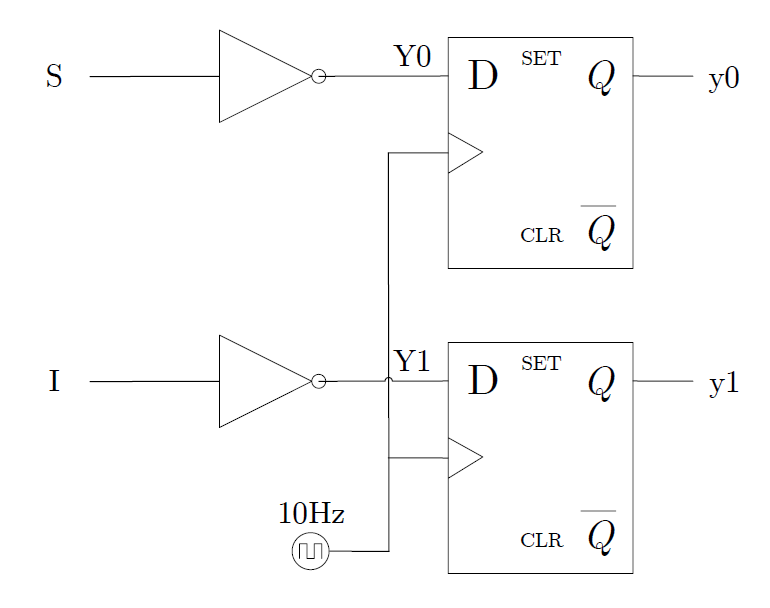
\includegraphics[scale=0.3]{images/input_moore.png}
\caption{Lógica de transición de estados}
\label{1_fig4}
\end{figure}

Para implementar la lógica combinacional de las salidas en función de los estados actuales, se decidió utilizar un multiplexor, de forma que por un lado se implemente la lógica que controle las salidas cuando éstas son iguales (estados \emph{Ninguna} y \emph{Ambas}) y por otro la lógica cuando las salidas deben ser complementarias (estado \emph{Una Sola}).

Para decodificar el estado de la máquina implementada, y poder controlar el mutiplexor mencionado y la lógica combinacional de las salidas, se utilizó un decodificador  2-a-4 74HC139. Este integrado implementa un decodificador de salidas active LOW, de esta forma, puedo decodificar el estado actual de la máquina para el posterior uso en la lógica de salida.

Cuando la máquina se encuentra en el estado \emph{Una Sola}(\emph{Una Sola=1}), las salidas no solo son complementarias (una bomba está encendida y la otra apagada), sino que además cada vez que 'entro' y 'salgo' del estado en cuestión, las salidas se deben intercalar, como indica la consigna. Para lograr esto, se utilizó un Flip-Flop JK en modo Toggle (J=1, K=1). El Clock del Flip-Flop en cuestión es alimentado por la señal \emph{~(Una Sola)}, como indica la Figura \ref{1_fig3}.

\begin{figure}[H]
\centering
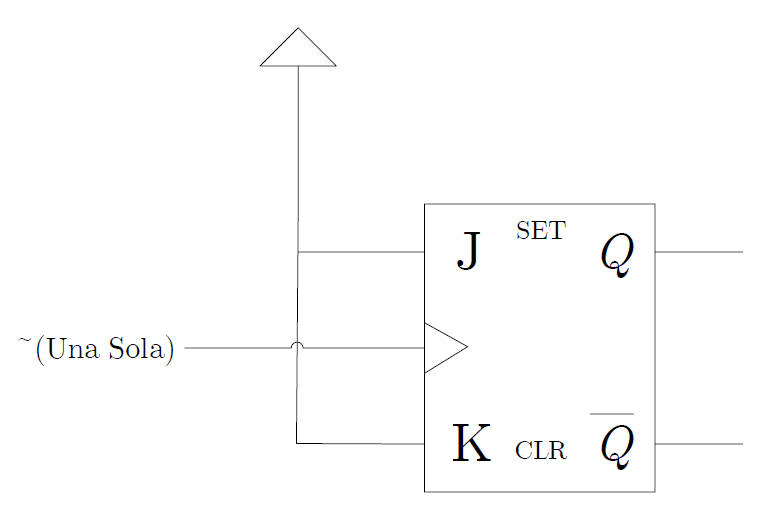
\includegraphics[scale=0.3]{images/jk_toggle_moore.png}
\caption{Flip-Flop JK para alternar salidas}
\label{1_fig3}
\end{figure}

Las salidas de este Flip-Flop alimentaron las entradas '0' de dos multiplexores como indica la Figura \ref{1_fig2}. De esta forma cuando la máquina se encuentre en el estado \emph{Una Sola}, las salidas $b_1$ y $b_2$ serán complementarias


\begin{figure}[H]
\centering
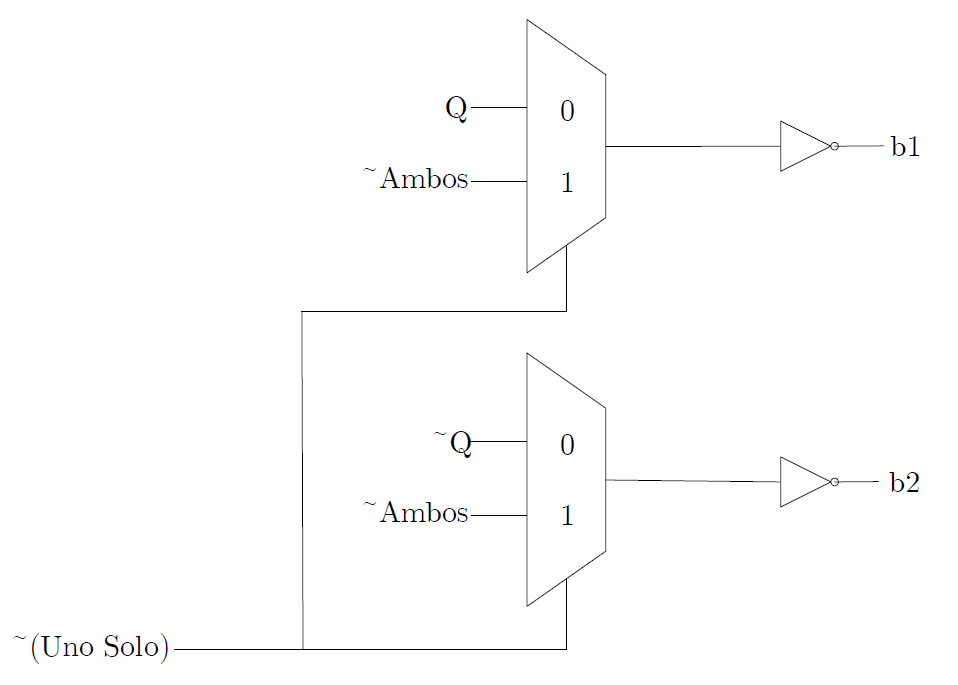
\includegraphics[scale=0.3]{images/multiplexion_moore.png}
\caption{Multiplexación a la salida}
\label{1_fig2}
\end{figure}

Por otro lado, cuando la máquina de estados se encuentre en el estado \emph{Ambos}, se seleccionará la entrada '1' del multiplexor, y obtendré un 1 a la salida de los mutiplexores cuando \emph{Ambos=0} y un 0 cuando  \emph{Ambos=1}. Como las salidas $b_1$ y $b_2$ son las salidas de los multiplexores negadas, entonces obtendremos $b_1b_2=11$ cuando \emph{Ambas=1} y $b_1b_2=00$ cuando \emph{Ambas=0}

El esquemático completo del circuito implementado en Altium Designer, a partir del cual se diseñó el circuito impreso se muestra en la Figura \ref{1_fig_esqm}.

\begin{figure}[ht]
\centering
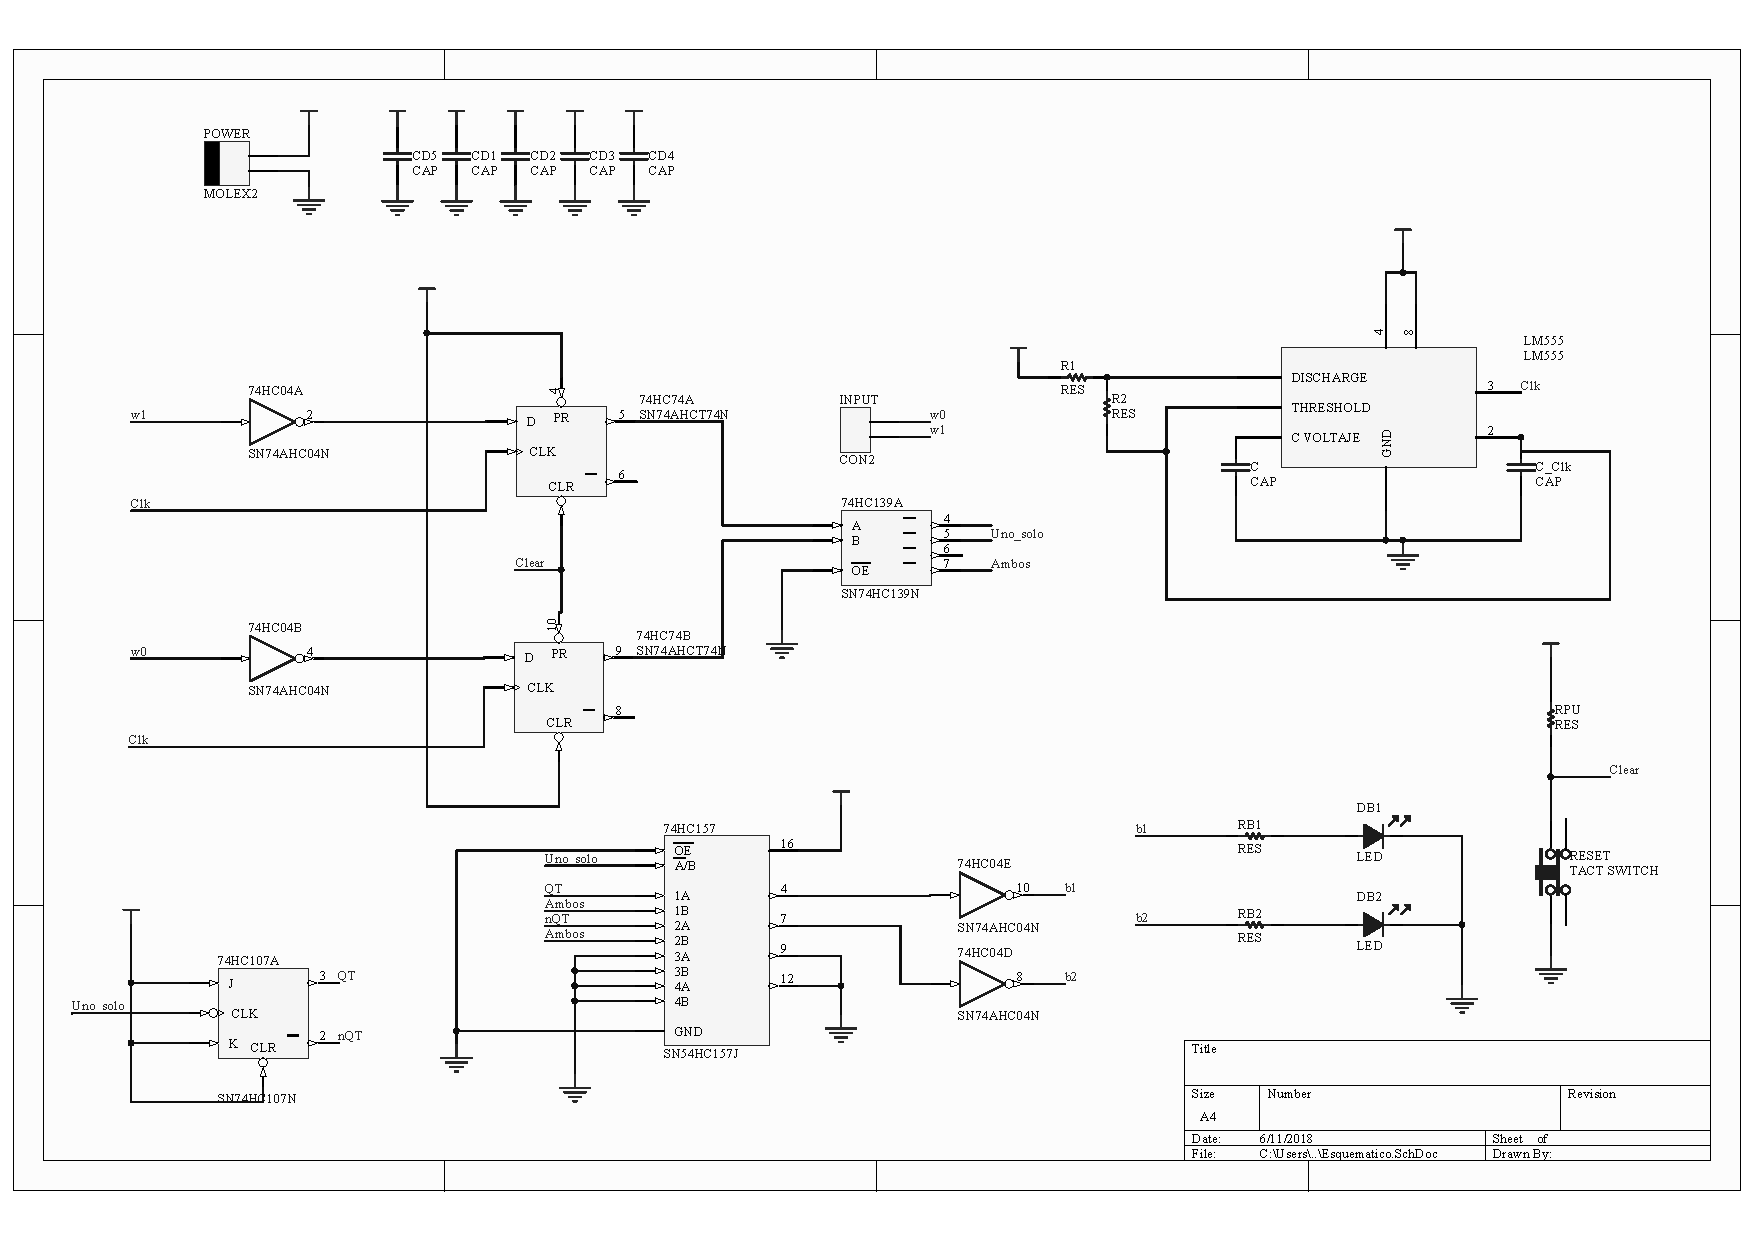
\includegraphics[scale=0.6]{images/Esquematico_Moore.pdf}
\caption{Esquemático del circuito implementado. Máquina de Moore}
\label{1_fig_esqm}
\end{figure}

\subsection*{Mediciones y Simulación}

En esta sección se contrastan las mediciones realizadas sobre el dispositivo implementado con los resultados arrojados por los códigos de Verilog que se encuentran disponibles en el repositorio. El diagrama de tiempo de las variables del modulo simulado se observan en la Figura \ref{1_fig_verilog_moore}.


\begin{figure}[H]
\centering
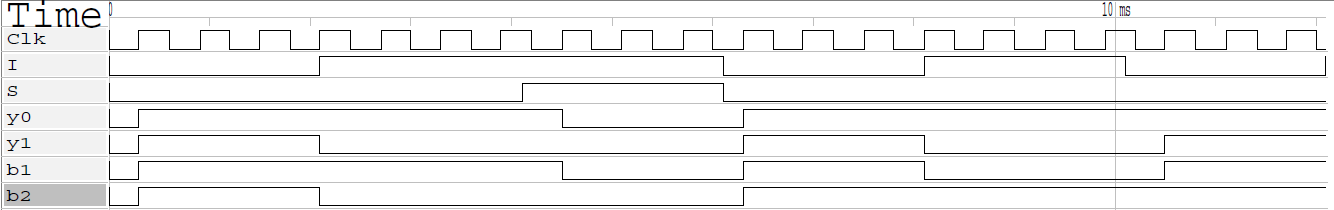
\includegraphics[scale=0.45]{images/time_diagram_moore}
\caption{Diagrama de tiempo simulado}
\label{1_fig_verilog_moore}
\end{figure}

El comportamiento de la simulación es el esperado, cumpliendo con los requerimientos de la consigna.

A continuación, en la figura \ref{1_fig_medicion_moore} se muestra una medición realizada sobre la placa implementada. En el mismo se muestran las entradas de los sensores I y S en los canales 3 y 4, y las salidas $b_1$ y $b_2$ en los canales 1 y 2. Como se mencionó anteriormente el caso S=1, I=0 se consideró como 'don't care', la medición muestra que para esta configuración de entrada ambas bombas están en estado 'apagadas'.

\begin{figure}[H]
\centering
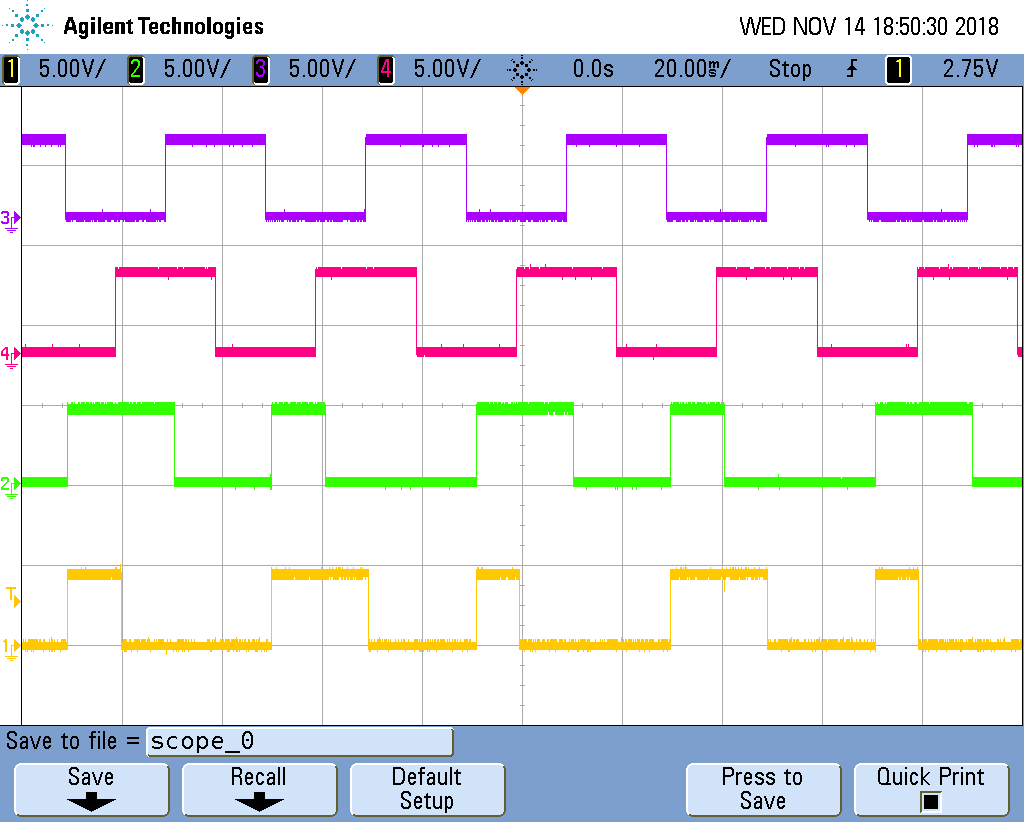
\includegraphics[scale=0.3]{images/medicion_ej1_moore}
\caption{Medición de entradas y salidas}
\label{1_fig_medicion_moore}
\end{figure}


\section*{Implementación Maquina de Mealy}
\subsection*{Diagrama de Estados y Transiciones}
Al igual que en el proceso de diseño de la máquina de estados de Moore, el primer paso fue determinar los estados de la máquina de estados. Las entradas y salidas son las mismas que para la máquina de Moore.

\subsubsection*{Estados:}

\begin{description}
\item[Juntas:] Estado que indica que ambas bombas están en el mismo estado, así sea encendidas o apagadas.
\item[Complementarias:] Estado que indica que los estados de las bombas son complementarios, es decir, una encendida y la otra apagada.
\end{description}

\begin{table}[H]
	\centering
	\begin{tabular}{c|c}
	y & Estado \\ 
	\hline 
	0 & Complementarias \\
	1 & Juntas \\ 
	\end{tabular} 
\end{table}

Al solamente necesitar de dos estados, puedo representarlos utilizando solamente una variable: $y$. El diagrama de estados de la máquina de Mealy se muestra en la Figura \ref{1_fig_estados_mealy}.


\begin{figure}[H]
\centering
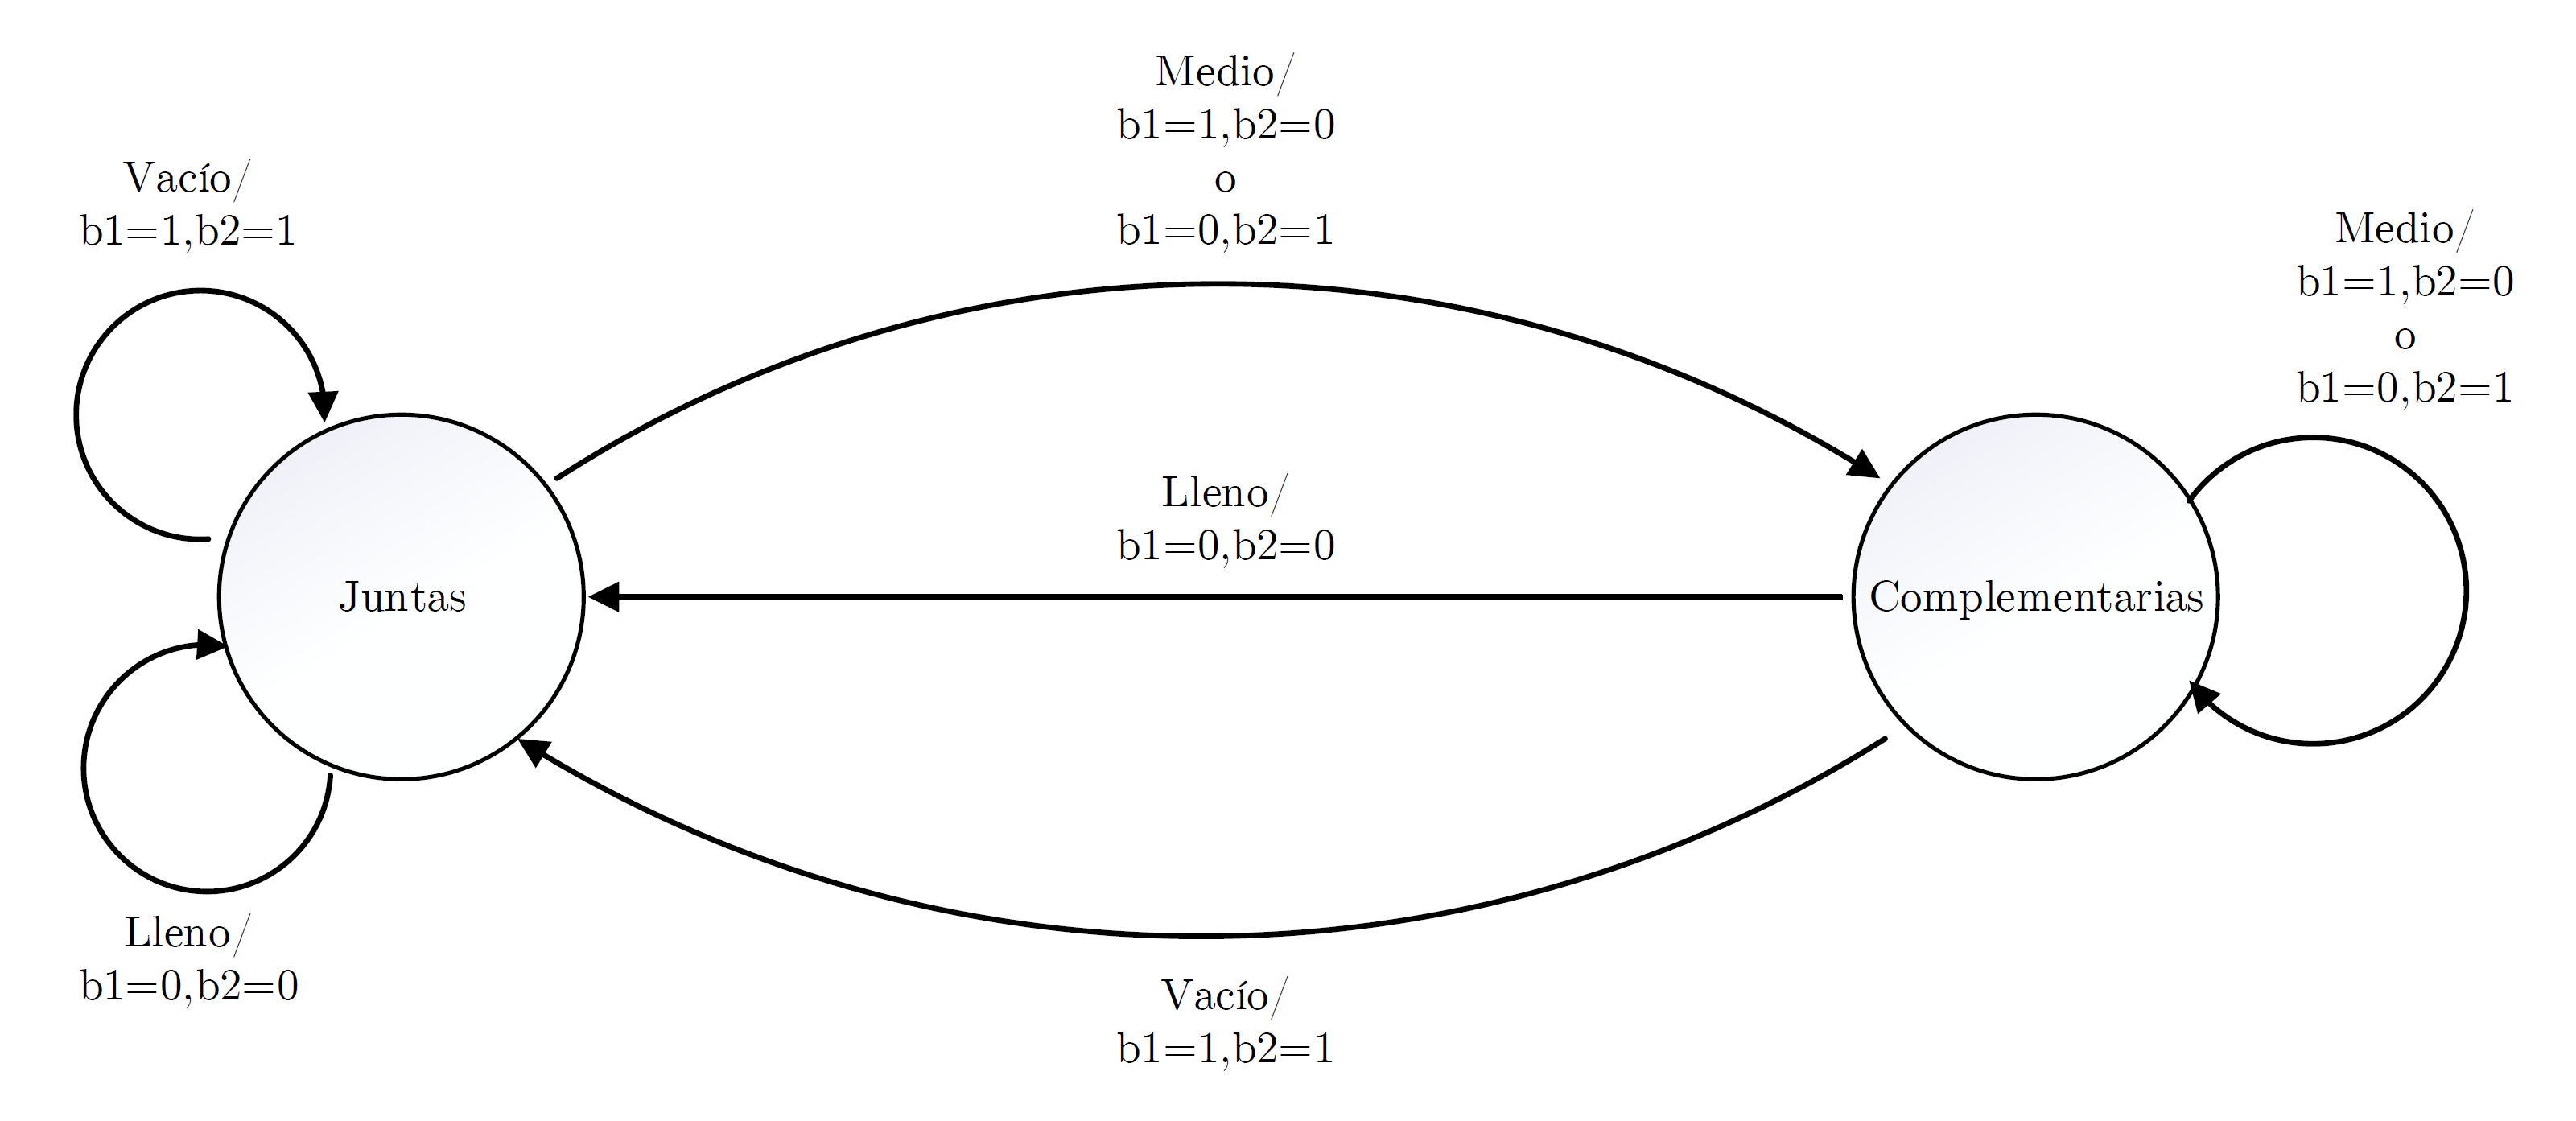
\includegraphics[scale=0.4]{images/diagrama_estados_mealy.png}
\caption{Diagrama de estados y transiciones} \label{1_fig_estados_mealy}
\end{figure}

Con el diagrama de estados definido, se completo la tabla de asignación de estados, representada en el Cuadro \ref{1_tabla_mealy_estados}.

\begin{table}[ht]
	\centering
	\begin{tabular}{c|c|c|c|c|c|c|c}
	Estado Actual & \multicolumn{3}{c|}{Próximo Estado$(Y)$} & \multicolumn{3}{c|}{Salida($b_1b_2$)}\\
	\cline{2-7}
	$(y)$ & $SI=00$ & $SI=01$ & $SI=11$ & $SI=00$ & $SI=01$ & $SI=11$ \\
	\hline
	0 & 1 & 0 & 0 & 11 & 10 o 01 & 00 \\
	1 & 1 & 0 & 0 & 11 & 10 o 01 & 00\\
	\end{tabular}
	\caption{Tabla de asignación de estados} \label{1_tabla_mealy_estados}
\end{table}

Al igual que se procedió en el caso de la máquina de Moore, a partir del Cuadro \ref{1_fig_estados_mealy} se confeccionó el Cuadro \ref{1_tabla_verdad_mealy}, que implementa la tabla de verdad que determina el próximo estado ($Y$) y las salidas($b_1b_2$) en función del estado anterior ($y$) y las entradas ($SI$). 

\begin{table}[H]
	\centering
	\begin{tabular}{c|c|c}
	$ySI$ & $Y$ & $b_1b_2$ \\ 
	\hline 
	000 & 1 & 11  \\ 
	\hline 
	001 & 0 & xx  \\ 
	\hline 
	010 & x & xx  \\ 
	\hline 
	011 & 1 & 00  \\ 
	\hline 
	100 & 1 & 11  \\ 
	\hline 
	101 & 0 & xx  \\ 
	\hline 
	110 & x & xx  \\ 
	\hline 
	111 & 1 & 00  \\ 
	\end{tabular} 
	\caption{Tabla de verdad cambio de estado} \label{1_tabla_verdad_mealy}
\end{table}

Cabe destacar que en la tabla de verdad del Cuadro \ref{1_tabla_verdad_mealy}, las salidas se definen como 'don't care'(x) para las configuraciones de entradas $ySI = x01$ y $ySI = x10$, esto es porque al igual que en la máquina de Moore, se utilizará un multiplexor y un Flip-Flop JK en modo Toggle (J=1, K=1) para seleccionar que las salidas sean iguales o complementarias.

Se simplificaron las funciones mediante mapas de Karnaugh, arrojando los siguientes resultados:

\begin{multicols}{2}
\begin{center}
\begin{Karnaughvuit}
	\minterms{0,4}
	\maxterms{3,7}
	\indeterminats{1,2,5,6}
	\implicant{0}{5}{}
\end{Karnaughvuit}

$b_1 = \overline{S}$, $b_2 = \overline{S}$
\end{center}

\columnbreak

\begin{center}
\begin{Karnaughvuit}
	\minterms{0,3,4,7}
	\maxterms{1,5}
	\indeterminats{2,6}
	\implicant{3}{6}{green}
	\implicantcostats{0}{6}{}
\end{Karnaughvuit}
\end{center}

\[
Y = S + \overline{I} = \overline{\overline{S}I}
\]
\end{multicols}

\subsection*{Implementación}

Se utilizó un Flip-Flop D para representar los dos estados de la maquina de Mealy, siguiendo los resultados arrojados por las tablas de verdad y los mapas de Karnaugh del apartado anterior. La Figura \ref{1_input_mealy} muestra el diagrama implementado.

\begin{figure}[H]
\centering
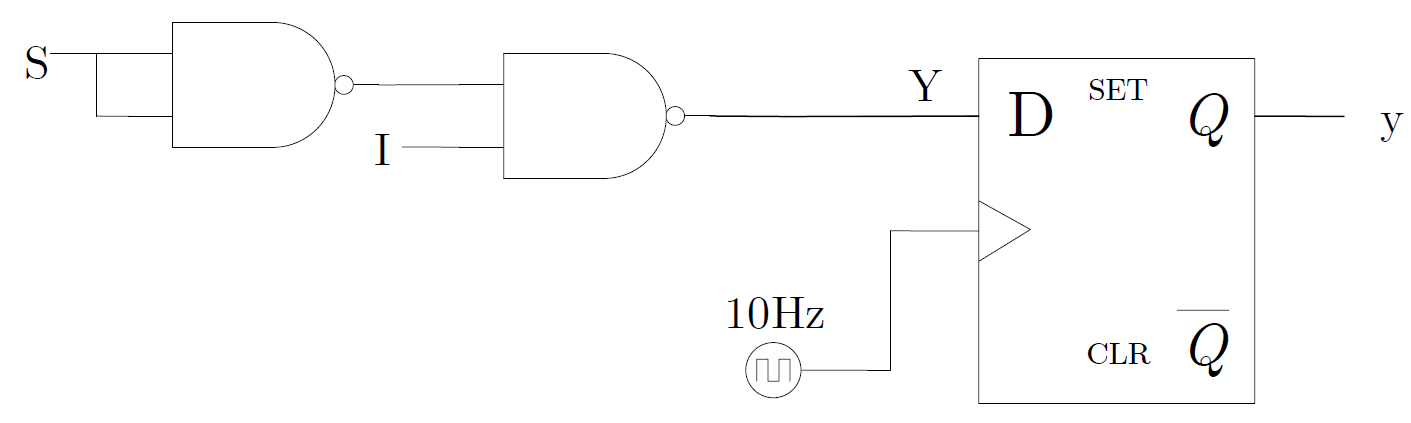
\includegraphics[scale=0.3]{images/input_mealy.png}
\caption{Lógica de transición de estados}
\label{1_input_mealy}
\end{figure}

La Figura \ref{1_salida_mealy} muestra la lógica implementada a la salida de la máquina de Mealy:

\begin{figure}[H]
\centering
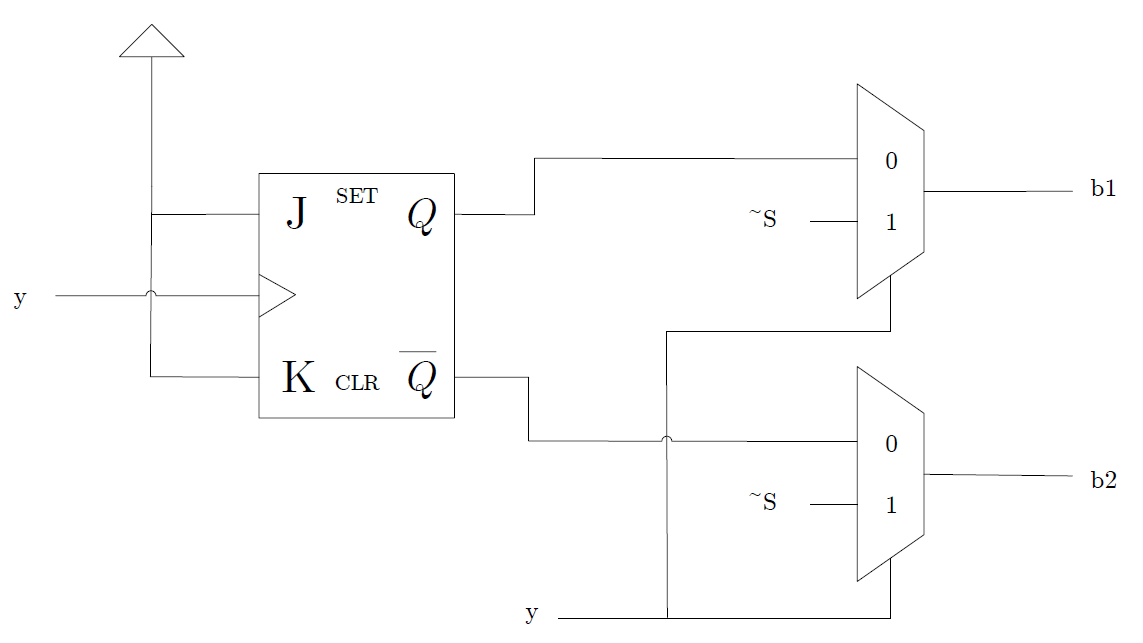
\includegraphics[scale=0.3]{images/multiplexion_mealy.png}
\caption{Lógica a la salida}
\label{1_salida_mealy}
\end{figure}

Al igual que en la máquina de Moore, el Flip-Flop JK togglea sus salidas cada vez que la variable de estados $y$ cambia de 0 a 1, es decir, cada vez que las bombas dejan de trabajar de forma complementaria. Las dos salidas del Flip-Flop alimentan la entrada '0' del multiplexior. Las entradas '1' de los mismos estan alimentadas por la señal $\overline{S}$. Las lineas de selección de los multiplexores están controladas por la variable de estado $y$. De esta forma cuando $y=0$ )(bombas complementarias), a la salida de los multiplexores obtengo las salidas complementarias del Flip-Flop JK. Por otro lado cuando $y=1$(ambas bombas trabajan juntas) obtengo a la salida de los multiplexores la señal $\overline{S}$, entonces cuando el depósito este lleno ($S=1$) obtendré en ambas salidas $\overline{1}=0$, es decir estarán apagadas. Cuando el deposito esté vacío la máquina esta en el estado $y=1$ y las entradas indicaran $SI=00$, entonces tendré en las salidas $\overline{0}=1$, es decir ambas bombas estarán encendidas.

El esquemático completo del circuito implementado en Altium Designer, a partir del cual se diseñó el circuito impreso se muestra en la Figura \ref{1_fig_esqm_mealy}.

\begin{figure}[ht]
\centering
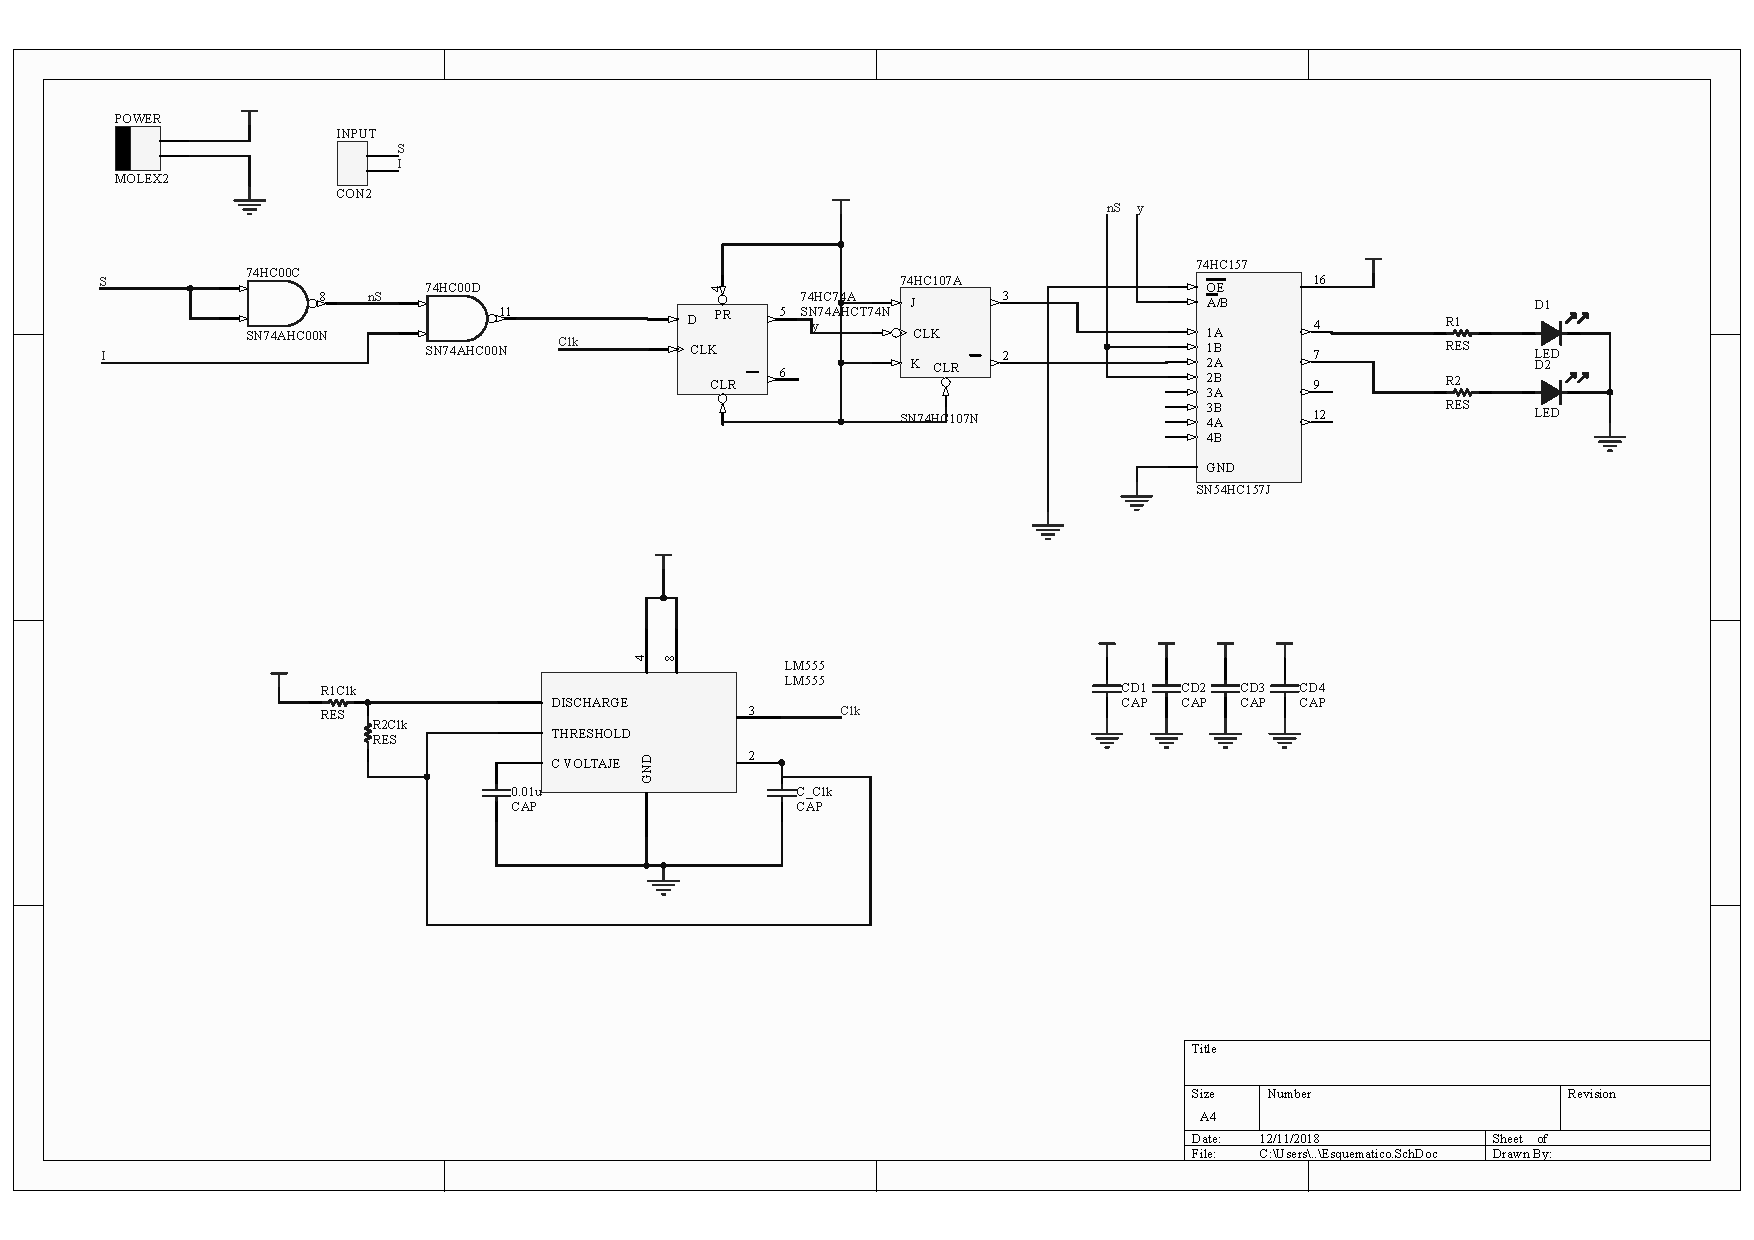
\includegraphics[scale=0.6]{images/Esquematico_Mealy.pdf}
\caption{Esquemático del circuito implementado. Máquina de MEaly}
\label{1_fig_esqm_mealy}
\end{figure}

\subsection*{Mediciones y Simulación}

En esta sección se contrastan las mediciones realizadas sobre el dispositivo implementado con los resultados arrojados por los códigos de Verilog que se encuentran disponibles en el repositorio. El diagrama de tiempo de las variables del modulo simulado se observan en la Figura \ref{1_fig_verilog_mealy}.


\begin{figure}[H]
\centering
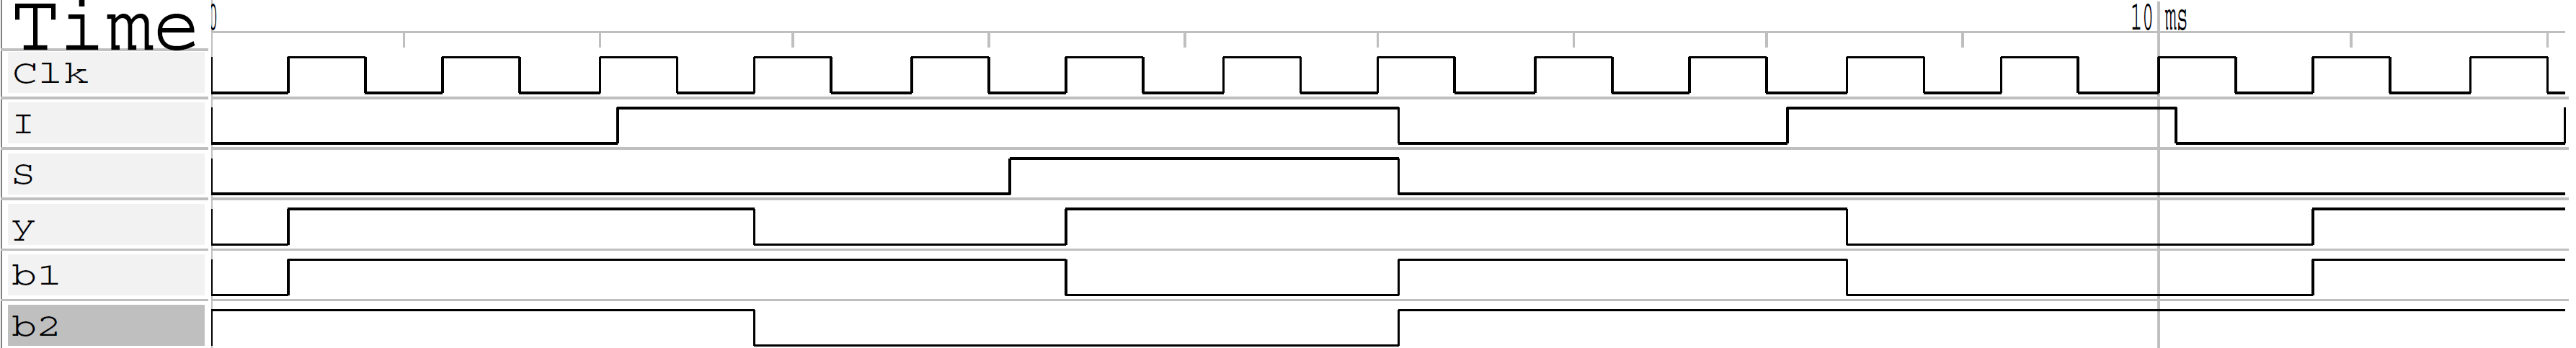
\includegraphics[scale=0.35]{images/time_diagram_mealy}
\caption{Diagrama de tiempo simulado}
\label{1_fig_verilog_mealy}
\end{figure}

El comportamiento de la simulación es el esperado, cumpliendo con los requerimientos de la consigna.

A continuación, en la figura \ref{1_fig_medicion_moore} se muestra una medición realizada sobre la placa implementada. En el mismo se muestran las entradas de los sensores S e I en los canales 3 y 4 respectivamente, y las salidas $b_1$ y $b_2$ en los canales 1 y 2. Como se mencionó anteriormente el caso S=1, I=0 se consideró como 'don't care' y la medición al igual que en la máquina de Moore, la máquina de Mealy muestra como salida $b_1b_2=00$ para el caso mencionado.

\begin{figure}[H]
\centering
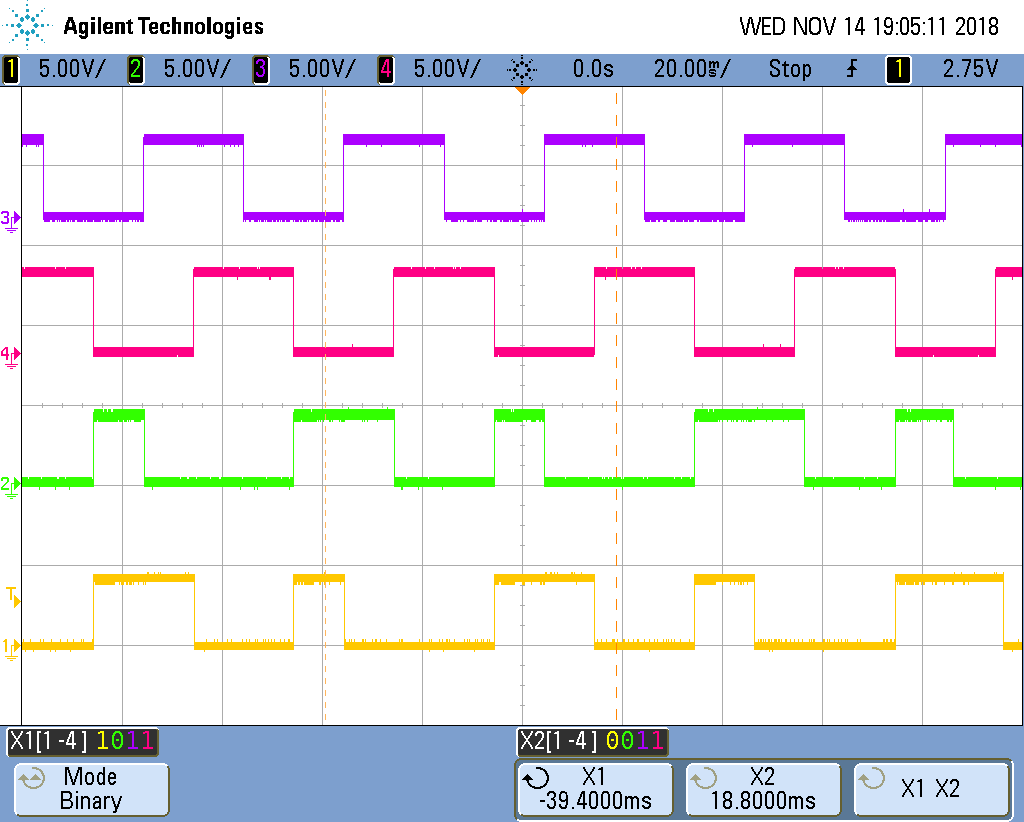
\includegraphics[scale=0.3]{images/medicion_ej1_mealy}
\caption{Medición de entradas y salidas}
\label{1_fig_medicion_mealy}
\end{figure}